\chapter{Resultados}
\label{chap:resultados}

Nesse capítulo serão apresentados os custos de produção para o hardware projetado, autonomia alcançada quando do uso de baterias e estratégias de uso dos recursos disponíveis para se otimizar a autonomia atual do projeto.

\section{Produção}

Foi realizado o levantamento dos custos, desde listas de materiais a custos de importação do hardware projetado, para algumas determinadas quantidades a fim de determinar seu preço unitário final para o consumidor.

\subsection{Lista de Materiais}

Tendo sido realizado todo o desenvolvimento da placa, foi criado a \textit{bill of materials - BOM} (lista de materiais) do hardware final. Nessa lista, para cada componente, foi descrito a quantidade utilizada, seu preço unitário e o valor resultante para a quantidade necessária desse componente. À partir desses valores, é possível inferir qual o custo total de aquisição dos componentes necessários para a fabricação de uma unidade do hardware proposto. 

Visando otimizar esse custo foi tomado como principal distribuidor de componentes eletrônicos a empresa LCSC Electronics, por conseguir oferecer os menores valores dentre os principais distribuidores de componentes eletrônicos do mercado. 

Assim, para a maioria dos componentes eletrônicos do hardware proposto foi possível encontrar uma opção nesse distribuidor. Dessa forma, o custo total da lista de materiais para a produção de determinadas unidades é o que segue:

	\begin{table}[!h]
	\captionsetup{width=7cm}%Deixe da mesma largura que a tabela
	\Caption{\label{tab:custos_fabricacao} Custo de materiais por unidades}%
	\IBGEtab{}{%
		\begin{tabular}{cccc}
			\toprule
			Quantidade & Custo de Materiais  \\
			\midrule \midrule
			50 &  US\$ 502,60  \\
			100 &  US\$ 938,41 \\
			1000 & US\$ 8.736,80  \\
			\bottomrule
		\end{tabular}%
	}{%
	\Fonte{o autor.}%
% 	\Nota{esta é uma nota, que diz que os dados são baseados na
% 		regressão linear.}%
% 	\Nota[Anotações]{uma anotação adicional, seguida de várias outras.}%
    }
    \end{table}





\subsection{Otimização de lista de materiais}

Para alguns componentes foram feitas recomendações tanto para quando da ocorrência da dificuldade de encontrar itens com os mesmos parâmetros nos distribuidores, quanto para necessidade de uma otimização do custo total da lista de materiais.

Os componentes D700 e D701 podem ser substituídos por equivalentes desde que as seguintes especificações sejam mantidas:
    \begin{itemize}
        \item Diâmetro da lente de 5mm;
        \item Montagem PTH;
        \item Tensão de operação de mínimo 1,8 V;
        \item Corrente de operação de no máximo 40 mA.
    \end{itemize}
    
  Os resistores R600, R601 e R602, por sua vez, atuam como resistores de \textit{pull-up} na comunicação com o cartão microSD. Devido isso, caso seja necessário, podem ser substituídos por resistores equivalentes com resistência entre 3,3 k$\Omega$ e 10k$\Omega$, potência igual ou superior a 1/16 W e encapsulamento SMD 0805.
    
 Há também a possibilidade de substituição do fusível rearmável F300 por um componente com o mesmo encapsulamento SMD 1206, corrente de \textit{trip} de 750 mA e tensão máxima igual ou superior a 6,5 V.
    
Por fim há o suporte para pilhas AA, que pode ser substituído por suportes semelhantes desde que mantenha as dimensões aproximadas de 53,34 mm X 50,80 mm, conecte até 4 pilhas AA em série e possua fios de que permitam conexão com o hardware proposto.

\subsection{Fabricação, montagem e custo unitário}

Um levantamento dos custos de fabricação e montagem dos componentes do hardware foi realizado junto a empresa JLCPCB, especialista em fabricação de placas de circuito impresso e que também oferece serviços de montagem dessas placas. Optou-se por essa fabricante devido sua parceria com o distribuidor LCSC Electronics para o fornecimento dos componentes necessários caso seja necessário ser realizado o processo de montagem de componentes da placa de circuito impressa produzida.

O processo de levantamento de custos com essa fabricante se deu pela disponibilização dos arquivos \textit{gerber} e lista de materiais do hardware projetado em sua plataforma digital e foram informados alguns parâmetros como a espessura da placa, material de fabricação e tipo de solda a ser usada. Em seguida, após alguns ajustes finais do processo de montagem de componentes, foi criado um orçamento para ambos os processos. Foram então levantados os valores de custo desses processos para as quantidades de 50, 100 e 1000 unidades, sendo obtidos os seguintes resultados:

	\begin{table}[!h]
	\captionsetup{width=7cm}%Deixe da mesma largura que a tabela
	\Caption{\label{tab:custos_fabricacao} Custos de fabricação e montagem JLCPCB}%
	\IBGEtab{}{%
		\begin{tabular}{cccc}
			\toprule
			Quantidade & Fabricação & Montagem & Total \\
			\midrule \midrule
			50 &  US\$ 22,4 & US\$ 64,47 & US\$ 86,87 \\
			100 &  US\$ 34,4 & US\$ 96,97 & US\$ 131,37 \\
			1000 & US\$ 249,70 & US\$ 447,92 & US\$ 667,62 \\
			\bottomrule
		\end{tabular}%
	}{%
	\Fonte{o autor.}%
% 	\Nota{esta é uma nota, que diz que os dados são baseados na
% 		regressão linear.}%
% 	\Nota[Anotações]{uma anotação adicional, seguida de várias outras.}%
    }
    \end{table}
% \newpage
Tendo sido levantado esses custos de fabricação e montagem, foi feito o custo total somando esses custos ao valor da lista de materiais para cada quantidade desejada, o que tornou possível estabelecer o custo unitário do hardware das placas fabricadas e montadas:


	\begin{table}[!h]
	\captionsetup{width=7cm}%Deixe da mesma largura que a tabela
	\Caption{\label{tab:custos_fabricacao} Custos de total unitário}%
	\IBGEtab{}{%
		\begin{tabular}{cccc}
			\toprule
			Quantidade & Custo Total & Custo Unitário  \\
			\midrule \midrule
			50 &  US\$ 582,42 & US\$ 11,65 \\
			100 &  US\$ 1048,93 & US\$ 10,49  \\
			1000 & US\$ 9261,29 & US\$ 9,26  \\
			\bottomrule
		\end{tabular}%
	}{%
	\Fonte{o autor.}%
% 	\Nota{esta é uma nota, que diz que os dados são baseados na
% 		regressão linear.}%
% 	\Nota[Anotações]{uma anotação adicional, seguida de várias outras.}%
    }
    \end{table}


\subsection{Custos de importação e valor unitário}

Devido a necessidade da fabricação no exterior, o processo de importação do hardware produzido acarreta em alguns custos para nacionalização do produto, sendo o primeiro deles o valor do transporte até o território brasileiro. Segundo ferramente de solicitação de fabricação da JLCPCB, o custo para o hardware projetado são os que seguem:

	\begin{table}[!h]
	\captionsetup{width=7cm}%Deixe da mesma largura que a tabela
	\Caption{\label{tab:custos_fabricacao} Custos de transporte para o Brasil}%
	\IBGEtab{}{%
		\begin{tabular}{cc}
			\toprule
			Quantidade & Valor  \\
			\midrule \midrule
			50 &  US\$ 80,36   \\
			100 &  US\$ 110,52 \\
			1000 & US\$ 524,49 \\
			\bottomrule
		\end{tabular}%
	}{%
	\Fonte{o autor.}%
	}
	\end{table}


À partir dos custos de transporte é possível fazer o cálculo das tarifas alfandegárias para a nacionalização do produto importado. Assim, para fins de auxílio nesse levantamento, foi tomado como destino o estado Ceará para cálculo da alíquota do \gls{ICMS}, e taxa de câmbio de R\$ 5,13 em relação ao dólar estadunidense. Vale ressaltar ainda que devido a decreto do Ministério da Economia do Brasil, \citeonline{dou2022}, a taxa de importação para equipamentos de informática e telecomunicações foi zerada e assim deve se manter até 31 de dezembro de 2025. Dessa forma, os custos alfandegários, total e final são discriminados abaixo, com todos os valores estando em reais:


	\begin{table}[!h]
	\captionsetup{width=10cm}%Deixe da mesma largura que a tabela
	\Caption{\label{tab:custos_fabricacao} Custos de importação para o Brasil}
	\IBGEtab{}{%
		\begin{tabular}{ccccccccc}
			\toprule
			Quantidade & Valor & Frete & IPI & PIS & COFINS & ICMS & Total & Valor Unitário  \\
			\midrule \midrule
            50   & 2.576,22  & 412,35   & 38,85  & 62,76  & 288,40   & 741,64    & 4.120,22  & 82,40 \\
            100  & 4.815,26  & 567,11   & 69,97  & 113,03 & 519,40   & 1.335,68  & 7.420,46  & 74,20 \\
            1000 & 44.831,14 & 2.691,32 & 617,79 & 997,97 & 4.585,92 & 11.793,10 & 65.517,24 & 65,52\\
			\bottomrule
		\end{tabular}%
	}{%
	\Fonte{o autor.}%
	}
	\end{table}





























\section{Energia}

A autonomia do uso da bateria no hardware proposto depende não só das funcionalidades de gerenciamento do consumo de energia oferecidas do módulo microcontrolador, como também de estratégias firmware que visem diminuir o consumo quando o hardware não estiver sendo totalmente utilizado. 

\subsection{Consumo energético dos circuitos}

Para mensurar o consumo energético total do hardware, foi necessário analisar seus componentes individualmente, sendo realizado uma análise por cada circuito que compõe o hardware. Tomou-se a interface de usuário como primeiro circuito a se analisar e foi notado que seus LEDs possuem um consumo típico de 30mA cada, enquanto os botões, por funcionarem como um fio condutor quando pressionados, não geram um consumo de corrente considerável. 

Em seguida analisou-se os circuitos dos sensores. Para o sensor de umidade e temperatura, segundo a folha de dados desse componente, seu consumo médio é de 1,3 $\mu$A para leituras constantes, com um pico de 7,2 mA somente quando a função de auto aquecimento é acionada. Contudo, caso nenhuma leitura esteja sendo feita, o sensor consome apenas 100 nA. Já o sensor de luminosidade não consome corrente por ser um componente passivo de resistência variável, deixando apenas que ela flua através de si.

No circuito do cartão microSD, o consumo depende das operações de leitura e escrita de dados. Essas operações consomem um máximo de 100mA cada quando o cartão estiver operando no modo padrão de velocidade, no qual é possível atingir uma taxa de transferência de até 12.5 MB/s \cite{2010sd3sd}. É também necessário o consumo de no máximo 1 mA para manter o cartão em estado de espera para realização de novas operações, o qual foi procurado eliminar ao oferecer a opção de desligar completamente o cartão microSD utilizando o transistor Q600 que no configuração atual funciona como uma chave na linha de alimentação do cartão.

Contudo se essa funcionalidade for utilizada e quando houver a necessidade de realizar novas operações, o processo de religamento do cartão microSD além do tempo mínimo de 250 milissegundos, é necessário também um consumo de no máximo 115 mA para que o cartão entre em estado de operação. 
% Para auxiliar na redução desse consumo energético, o componente Q600 foi introduzido na linha de alimentação do suporte de leitura de cartões microSD. Esse componente é um transistor MOSFET de canal P que foi escolhido para operar nos modos de corte e saturação de forma que seja possível controlar quando o cartão deverá ser alimentado, eliminando assim o seu consumo em modo de espera restando assim somente o consumo quando da realização de operações de leitura e escrita.

Para o circuito de controle foi necessário consultar a folha de dados do módulo microcontrolador, no qual a fabricante recomenda que haja um suprimento mínimo de 500mA de corrente para seu funcionamento, porém isso é necessário quando há o pleno funcionamento de todos os seus periféricos e dos rádios Wi-Fi e Bluetooth. Como o hardware proposto não fará uso de comunicação utilizando os rádios disponíveis, é possível configurar o módulo de forma a não usá-los e obter um consumo típico de 30 mA operando na frequência de 80 MHz. Junto a isso há ainda possibilidade de se escolher por meio de firmware um dos dois modos de operação de baixo consumo disponíveis, \textit{light-sleep} ou \textit{deep-sleep}. 

Naquele, o módulo microcontrolador reduz o clock de operação de sua CPU, memória RAM e periféricos, além de também reduzir a tensão de alimentação que lhes é fornecida, a operação de instruções na CPU é pausada em um determinado ponto e também há a opção de desativar totalmente alguns dos periféricos. O rádio Wi-Fi é capaz ainda de manter uma conexão ativa. Nesse modo, de acordo com a folha de dados da fabricante é possível atingir um consumo de 240 $\mu$A. 
% , contudo devido a características inerentes a construção do módulo e de  acordo com testes realizados pela fabricante, foi possível atingir um consumo médio de 1,3 mA em um contexto no o módulo alternava a cada 2 segundos entre esse modo e o modo de operação ativo. 

No modo \textit{deep-sleep} a CPU e a maioria dos periféricos do hardware são desligados, permanecendo ativos somente seu co-processador de baixíssima potência (\textit{Ultra-Low-Power} - ULP), periféricos e memória RTC. Esse estado se mantém enquanto não houver um evento, à partir das fontes determinadas em documentação, que leve ao co-processador a despertar a CPU e seus demais periféricos. Dessa forma, segundo sua folha de dados, o consumo médio nesse modo é de 8$\mu$A.

Assim, com base nos dados levantados, o consumo típico dos circuitos do hardware proposto, em miliampères, são resumidamente:

	\begin{table}[!h]
	\captionsetup{width=7cm}%Deixe da mesma largura que a tabela
	\Caption{\label{tab:consumos_circuitos} Consumo típico por circuito}%
	\IBGEtab{}{%
		\begin{tabular}{cc}
			\toprule
			Circuito & Consumo \\
			\midrule \midrule
			Controle  &  30  mA \\
			Sensores  &  0,0013 mA  \\
			MicroSD   &   100 mA\\
			Interface de Usuário & 60 mA\\
		    \bottomrule
		\end{tabular}%
	}{%
	\Fonte{o autor.}%
% 	\Nota{esta é uma nota, que diz que os dados são baseados na
% 		regressão linear.}%
% 	\Nota[Anotações]{uma anotação adicional, seguida de várias outras.}%
    }
    \end{table}

% \newpage
\subsection{Autonomia e estratégias de otimização}

% Em um cenário testado pela fabricante, no qual o módulo microcontrolador operou no modo \textit{light-sleep} durante dois segundos e em seguida foi alternado para o modo de operação ativo a 80 MHz durante 9 milissegundos, foi obtido um consumo médio de 1,3 mA.

Definir o tempo de autonomia real para o hardware proposto, depende de dados empíricos de consumo energético que não puderam ser levantados por não ter sido possível produzir unidades de teste desse hardware. Dessa forma, foi estimada uma autonomia com base nas especificações de consumo máximo dos componentes do hardware, descritos em suas folhas de dados e destacados na tabela \ref{tab:consumos_circuitos}. Assim, o consumo total do hardware proposto é de aproximadamente 190 mA quando houver sendo feito uso constante de todas as suas funcionalidades, possui uma autonomia típica de 13 h 9 min quando a alimentação for realizada por um conjunto de quatro pilhas AA em que cada possua uma capacidade de 2500 mAh, o que está aquém das especificações do projeto. Para otimizar esse tempo, é necessário a adoção de algumas estratégias quando do desenvolvimento do firmware para esse hardware.

Reduzir o tempo de utilização do cartão microSD por meio da diminuição do número de operações de escrita no cartão, deve ser uma das primeiras estratégias a serem consideradas e que pode ser realizada por meio da acumulação dos dados lidos dos sensores na memória flash do módulo microcontrolador em blocos de dados que seriam gravados no cartão microSD somente quando atingissem um tamanho pré-determinado. Essa estratégia pode ser otimizada com a utilização do transistor da linha de alimentação do cartão, que permite seu desligamento completo, eliminando assim o consumo em estado de espera durante o período que não houver operações de gravação de dados. 

A operação do módulo microcontrolador durante períodos maiores de tempo nos modos de operação com baixo consumo energético disponíveis, também se mostra como possível estratégia para economia energética. Em um cenário apresentado pela fabricante  no qual o módulo microcontrolador operou no modo \textit{light-sleep} durante dois segundos e em seguida foi alternado para o modo de operação ativo a 80 MHz durante nove milissegundos, foi obtido um consumo médio de 1,3 mA.







% \section{Arquivos de saída}

% \begin{itemize}
%     \item Arquivos de Fabricação
%     Grupo formado pelos arquivos gerber e lista de materiais da placa desenvolvida.
    
    
    
%     \item Arquivos de Montagem
    
%     Grupo formado pelos arquivos Pick and Place e documentos em PDF das silkscreens da placa.
    
    
%     \item Arquivos de Documentação
    
    
%     Grupo formado pela lista de materiais, esquemáticos eletrônicos, design PCB e visualização 3D compilados em um único documento PDF.
    

% \end{itemize}





% Texto texto texto texto texto texto texto texto texto texto texto texto texto texto texto texto texto texto texto texto texto texto texto texto texto texto texto texto texto texto texto texto texto texto texto texto texto texto texto texto texto texto texto texto texto texto texto texto texto texto texto texto texto texto texto texto texto texto texto texto texto texto texto texto texto texto texto texto texto.

% \section{Resultados do Experimento A}
% \label{sec:resultados-do-experimento-a}

% Procure deixar as figuras dos resultados o maior possível preenchendo a largura do texto do documento que possui $16~cm$.

% \begin{figure}[h!]
%         \captionsetup{width=16cm}
% 		\Caption{\label{fig:tensaoimpedanciahumana} Gráfico de tensão considerando a impedância humana}
% 		%\centering
% 		\UFCfig{}{
% 			\fbox{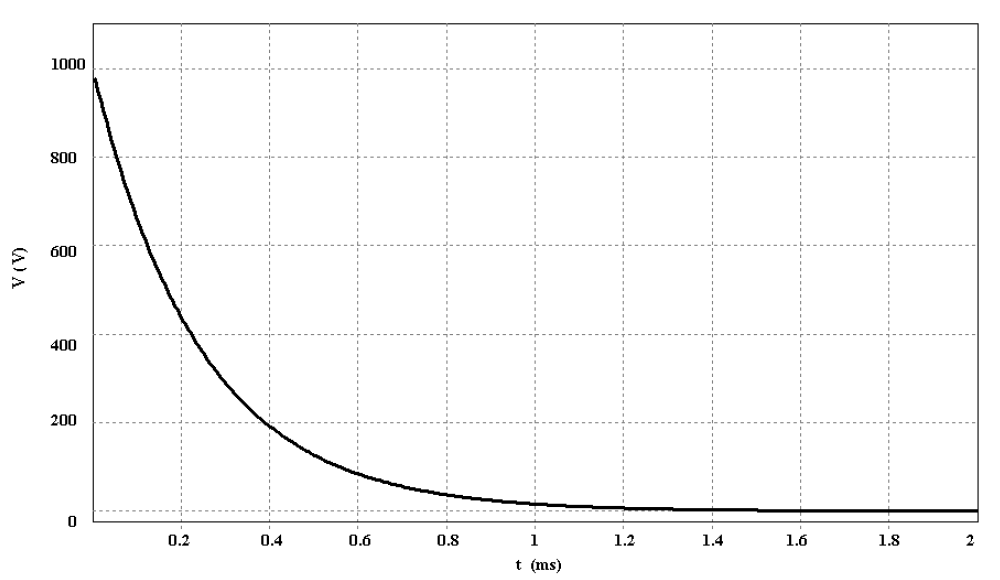
\includegraphics[width=16cm]{figuras/tensaoimpedanciahumana}}
% 		}{
% 			\Fonte{elaborado pelo autor (2016).}
% 		}	
% \end{figure}

% Texto texto texto texto texto texto texto texto texto texto texto texto texto texto texto texto texto texto texto texto texto texto texto texto texto texto texto texto texto texto texto texto texto texto texto texto texto texto texto texto texto texto texto texto texto texto texto texto texto texto texto texto texto texto texto texto texto texto texto texto texto texto texto texto texto texto texto texto texto.

% \begin{figure}[h!]
% 	\captionsetup{width=16cm}
% 	\Caption{\label{fig-grafico-1}Produção anual das dissertações de mestrado e teses de doutorado entre os anos de 1990 e 2008}		
% 	\IBGEtab{}{
% 		\fbox{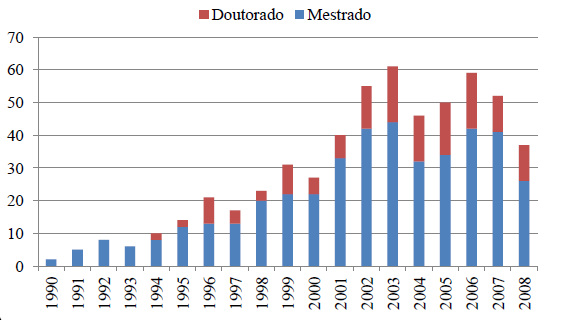
\includegraphics[width=16cm]{figuras/figura-3}}
% 	}{
% 	\Fonte{elaborado pelo autor (2016).}
% }
% \end{figure}

% Texto texto texto texto texto texto texto texto texto texto texto texto texto texto texto texto texto texto texto texto texto.

% Texto texto texto texto texto texto texto texto texto texto texto texto texto texto texto texto texto texto texto texto texto texto texto texto texto texto texto texto texto texto texto texto texto texto texto texto texto texto texto texto texto texto texto texto texto texto texto texto texto texto texto texto texto texto texto texto texto texto texto texto texto texto texto texto texto texto texto texto texto.

% \section{Resultados do Experimento B}
% \label{sec:resultados-do-experimento-b}

% Texto texto texto texto texto texto texto texto texto texto texto texto texto texto texto texto texto texto texto texto texto texto texto texto texto texto texto texto texto texto texto texto ..

% \begin{table}[h!]	
% 	%\centering
% 	\captionsetup{width=11.3cm}%ATENÇÃO: Ajuste a largura do título
% 	\Caption{\label{tab:notas} Notas dos participantes nas avaliações A, B e C}	
% 	\IBGEtab{}{
% 		\begin{tabular}{crrr}
% 			\toprule
% 			Identificação dos participantes & Avaliação A & Avaliação B &                        Avaliação C \\
% 			\midrule \midrule
% 			Participante 1 & 7 & 9 & 10\\
% 			Participante 2 & 8 & 2 & 1\\
% 			Participante 3 & 5 & 10 & 6 \\
% 			Participante 4 & 3 & 1 & 4\\
% 			Participante 5 & 2 & 4 & 1\\
% 			Participante 6 & 0 & 7 & 2\\
% 			\bottomrule
% 		\end{tabular}
% 	}{
% 	\Fonte{elaborado pelo autor (2016).}
% }
% \end{table}

%  Texto texto Referenciando a \autoref{tab:notas}  texto texto texto texto texto texto texto texto texto texto texto texto texto texto texto texto texto texto texto texto texto texto texto texto texto texto texto texto texto texto.Texto texto texto texto texto texto texto texto texto texto texto texto texto texto texto texto texto texto texto texto texto.

% Texto texto texto texto texto texto texto texto texto texto texto texto texto texto texto texto texto texto texto texto texto texto texto texto texto texto texto texto texto texto texto texto texto texto texto texto texto texto texto texto texto texto texto texto texto texto texto texto texto texto texto texto texto texto texto texto texto texto texto texto texto texto texto texto texto texto texto texto texto.Texto texto texto texto texto texto texto texto texto texto texto texto texto texto texto texto texto texto texto texto texto texto texto texto texto texto texto texto texto texto texto texto texto texto texto texto texto texto texto texto texto.

% Texto texto texto texto texto texto texto texto texto texto texto texto texto texto texto texto texto texto texto texto texto texto texto texto texto texto texto texto texto texto texto texto texto texto texto texto texto texto texto texto texto texto texto texto texto texto texto texto.Texto texto texto texto texto texto texto texto texto texto texto texto texto texto texto texto texto texto texto texto texto.

% Texto texto  Referenciando a \autoref{tab:notas}  texto texto texto texto texto texto texto texto texto texto texto texto texto texto texto texto texto texto texto texto texto texto texto texto texto texto texto texto texto texto texto texto texto texto texto texto texto texto texto texto texto texto texto texto texto texto texto texto texto texto texto texto texto texto texto texto texto texto texto texto texto texto texto texto texto texto texto.